\chapter*{Findings}
\begin{table}[htb]
    \renewcommand{\arraystretch}{1.5}
    \begin{tabular*}{\textwidth}{|>{\columncolor{red!15}}p{3cm}|p{17.1cm}|}
    \textbf{Finding} & \textbf{Root read access on port 433}\\
    Risk& High \\
    Category & Broken Access Control, Misconfiguration\\
    Impact& An attacker read access to all files on the server. This can also happen to regular users by accident.\\ 
    Description& 
    After trying to access the server on port 433 with the url https://172.16.0.29:433 an error message was displayed: \newline \newline
    Error opening ''
    548660451168:error:02001002:system library:fopen:No such file or directory:bss\_file.c:169:fopen('','r') \newline
    548660451168:error:2006D080:BIO routines:BIO\_new\_file:no such file:bss\_file.c:172:
    \newline
    After considering serveral option what the purpose of the \ac{https} service running on port 433 was, it turned out that it represents the file system of the server. It is possible to access serveral files on the server.
    \newline
    \newline
    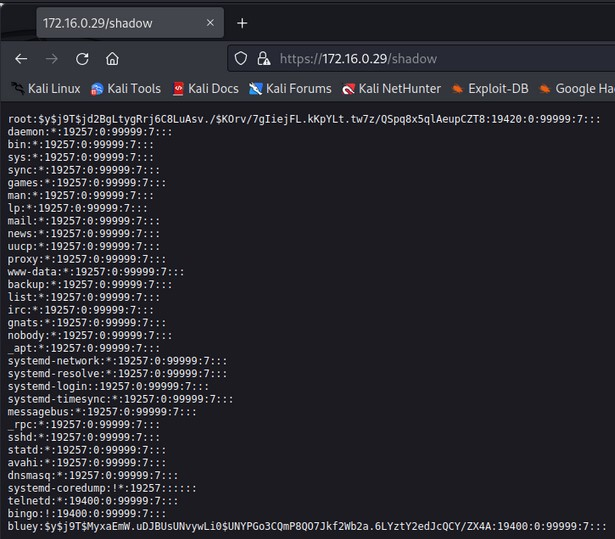
\includegraphics[width=0.73\textwidth]{Webserver_root_access.jpg}
    \newline
    Shown in the graphic above it was possible to access the shadow.txt file of the server where the hashes of all user passwords are listed.
	\\   
    \end{tabular*}
    \end{table}